\documentclass[12pt,a4paper,twoside]{article}

% ============================================================
% 哈尔滨工程大学本科生毕业论文 LaTeX 模板
% 严格按22级论文模板格式
% ============================================================

% 页面设置
\usepackage[top=28mm,bottom=28mm,left=25mm,right=25mm,headheight=30pt]{geometry}

% 字体和编码
\usepackage{times}
\usepackage[T1]{fontenc}
\usepackage[UTF8]{ctex}

% 图形和绘图
\usepackage{tikz}
\usetikzlibrary{calc,positioning}

% 行距设置
\usepackage{setspace}
\setstretch{1.3}

% 段落缩进
\setlength{\parindent}{2em}

% 章节标题格式
\usepackage{titlesec}

% 一级标题：小2号Times New Roman Bold，罗马数字，居中
\titleformat{\section}
  {\centering\fontsize{18pt}{22pt}\selectfont\bfseries}
  {\thesection}{1em}{}
\renewcommand{\thesection}{\Roman{section}}
\titlespacing*{\section}{0pt}{1\baselineskip}{1\baselineskip}

% 二级标题：小3号Times New Roman Bold
\titleformat{\subsection}
  {\fontsize{15pt}{22pt}\selectfont\bfseries}
  {\thesubsection}{1em}{}
\renewcommand{\thesubsection}{\arabic{section}.\arabic{subsection}}

% 三级标题：4号Times New Roman Bold
\titleformat{\subsubsection}
  {\fontsize{14pt}{22pt}\selectfont\bfseries}
  {\thesubsubsection}{1em}{}
\renewcommand{\thesubsubsection}{\arabic{section}.\arabic{subsection}.\arabic{subsubsection}}

% 页眉页脚设置
\usepackage{fancyhdr}
\pagestyle{fancy}
\fancyhf{}

% 双页页眉：哈尔滨工程大学本科生毕业论文
\fancyhead[CE]{\fontsize{10.5pt}{15.75pt}\selectfont 哈尔滨工程大学本科生毕业论文}
% 单页页眉：章标题（正文部分）
\fancyhead[CO]{\fontsize{10.5pt}{15.75pt}\selectfont \leftmark}
\fancyfoot[C]{\thepage}

% 页眉线：上细下粗（3磅=1.5pt）
\renewcommand{\headrule}{%
  \vspace{-2pt}
  
\begin{tikzpicture}
    \draw[line width=0.4pt] (0,0) -- (\textwidth,0);
    \draw[line width=3pt] (0,-2pt) -- (\textwidth,-2pt);
  \end{tikzpicture}
  \vspace{2pt}
}

% 定义前置部分页眉样式（摘要、目录）：只有页码，无页眉
\fancypagestyle{frontmatter}{%
  \fancyhf{}
  \fancyfoot[C]{\fontsize{10.5pt}{15pt}\selectfont \thepage}
  \renewcommand{\headrulewidth}{0pt}
  \renewcommand{\headrule}{}
}

% 定义后置部分页眉样式（Reference及以后）
\fancypagestyle{backmatter}{%
  \fancyhf{}
  \fancyhead[CE]{\fontsize{10.5pt}{15.75pt}\selectfont 哈尔滨工程大学本科生毕业论文}
  \fancyhead[CO]{\fontsize{10.5pt}{15.75pt}\selectfont Polar Route Planning and 3D Reconstruction Using Unreal Engine and 3D Gaussian Splatting}
  \fancyfoot[C]{\thepage}
  \renewcommand{\headrule}{%
    \vspace{-2pt}
    
\begin{tikzpicture}
      \draw[line width=0.4pt] (0,0) -- (\textwidth,0);
      \draw[line width=3pt] (0,-2pt) -- (\textwidth,-2pt);
    \end{tikzpicture}
    \vspace{2pt}
  }
}

% 章节标题标记
\renewcommand{\sectionmark}[1]{\markboth{\Roman{section}. \MakeUppercase{#1}}{}}

% 图表
\usepackage{graphicx}
\usepackage{caption}
\captionsetup{font=small,labelfont=bf}

% 图表编号按章编号
\renewcommand{\thefigure}{\arabic{section}.\arabic{figure}}
\renewcommand{\thetable}{\arabic{section}.\arabic{table}}
\makeatletter
\@addtoreset{figure}{section}
\@addtoreset{table}{section}
\makeatother

% 列表
\usepackage{enumitem}

% 数学公式
\usepackage{amsmath}
\usepackage{amssymb}

% 代码高亮
\usepackage{listings}
\lstset{
  basicstyle=\ttfamily\small,
  frame=single,
  breaklines=true,
  showstringspaces=false,
  keywordstyle=\color{blue},
  commentstyle=\color{green!50!black},
  stringstyle=\color{red},
  numbers=left,
  numberstyle=\tiny\color{gray},
  numbersep=8pt
}

% 参考文献
\usepackage[backend=biber,style=authoryear,natbib=true]{biblatex}
\addbibresource{references.bib}

% 超链接
\usepackage{hyperref}
\hypersetup{colorlinks=true,linkcolor=black,citecolor=black,urlcolor=blue}

% 表格
\usepackage{booktabs}
\usepackage{multirow}

% 颜色
\usepackage{xcolor}

% 目录格式设置
\usepackage{tocloft}
\renewcommand{\contentsname}{Contents}
\renewcommand{\cfttoctitlefont}{\hfill\bfseries}  % 标题加粗并居中
\renewcommand{\cftaftertoctitle}{\hfill}
\setlength{\cftbeforesecskip}{0.1em}  % 减小目录章节间距
\setlength{\cftbeforesubsecskip}{0.05em}  % 减小二级标题间距
\setlength{\cftbeforesubsubsecskip}{0.02em}  % 减小三级标题间距
% 确保所有级别都有虚线连接到页码
\renewcommand{\cftsecleader}{\cftdotfill{\cftdotsep}}
\renewcommand{\cftsubsecleader}{\cftdotfill{\cftdotsep}}
\renewcommand{\cftsubsubsecleader}{\cftdotfill{\cftdotsep}}
\renewcommand{\cftsecpagefont}{\bfseries}  % 章节页码加粗（与标题一致）
\setlength{\cftsecindent}{0pt}  % 章节不缩进
\setlength{\cftsubsecindent}{1em}  % 二级标题缩进
\setlength{\cftsubsubsecindent}{2em}  % 三级标题缩进
\setlength{\cftaftertoctitleskip}{1em}  % 标题后间距
\setlength{\cftbeforetoctitleskip}{-0.5em}  % 标题前间距

% ============================================================
% 文档开始 - 严格按模板顺序
% ============================================================
\begin{document}

% ===== 1. 英文封面 (无页码) =====
% ============================================================
% 英文封面 (English Cover) - Page 1
% ============================================================
\begin{titlepage}
\thispagestyle{empty}
\begin{center}

\vspace*{0.5cm}

% Student ID（右对齐）
\begin{flushright}
\fontsize{12pt}{18pt}\selectfont
Student ID\quad\underline{\makebox[5cm]{2022XXXXXXXX}}
\end{flushright}

\vspace{1.5cm}

% 学校名称
{\fontsize{18pt}{27pt}\selectfont Harbin Engineering University}\\[0.5cm]
{\fontsize{16pt}{24pt}\selectfont Undergraduate Students Individual Project Report}

\vspace{3cm}

% 英文题目（2号Times New Roman Bold）
{\fontsize{18pt}{27pt}\selectfont\bfseries
Polar Route Planning and 3D Reconstruction\\[0.3cm]
Using Unreal Engine and 3D Gaussian Splatting}

\vspace{4cm}

% 信息表格（左对齐标签）
\begin{flushleft}
\hspace{2cm}
\begin{tabular}{rl}
\fontsize{14pt}{21pt}\selectfont College: & \fontsize{14pt}{21pt}\selectfont Southampton Ocean Engineering Joint Institute \\[0.4cm]
\fontsize{14pt}{21pt}\selectfont Program Title: & \fontsize{14pt}{21pt}\selectfont Naval Architecture and Ocean Engineering \\[0.4cm]
\fontsize{14pt}{21pt}\selectfont Student Name: & \fontsize{14pt}{21pt}\selectfont Zhang Shihao \\[0.4cm]
\fontsize{14pt}{21pt}\selectfont Supervisor: & \fontsize{14pt}{21pt}\selectfont Associate Prof. Xing Xianglei / Prof. Dominic Taunton \\[0.4cm]
\fontsize{14pt}{21pt}\selectfont Word count: & \fontsize{14pt}{21pt}\selectfont 8087 \\
\end{tabular}
\end{flushleft}

\vfill

% 底部学校名称和日期
{\fontsize{14pt}{21pt}\selectfont Harbin Engineering University}\\[0.5cm]
{\fontsize{14pt}{21pt}\selectfont May, 2026}

\end{center}
\end{titlepage}


% ===== 2. 中文封面 (无页码) =====
% ============================================================
% 中文封面 (Chinese Cover) - 严格按照哈尔滨工程大学模板，单页
% ============================================================
\begin{titlepage}
\thispagestyle{empty}

% 学号、密级（右上方）
\vspace*{0.8cm}
\begin{flushright}
\fontsize{12pt}{18pt}\selectfont
学\hspace{0.5em}号\underline{\makebox[4cm]{2022XXXXXXXX}}\hspace{1cm}\\[0.2cm]
密\hspace{0.5em}级\underline{\makebox[4cm]{公开}}\hspace{1cm}
\end{flushright}

\vspace{1.5cm}

\begin{center}

% 学校名称（小2号）
{\fontsize{18pt}{27pt}\selectfont 哈尔滨工程大学本科生毕业论文}

\vspace{2.5cm}

% 论文题目（2号黑体加粗）
{\fontsize{22pt}{33pt}\selectfont\bfseries
基于 Unreal Engine 和 3D Gaussian Splatting 的\\[0.5cm]
极地路径规划与三维重建}

\vspace{3.5cm}

% 信息栏（4号）
\fontsize{14pt}{22pt}\selectfont
\begin{tabular}{r@{：}l}
学\hspace{1em}院\hspace{1em}名\hspace{1em}称 & 南安普顿海洋工程联合学院 \\[0.5cm]
专\hspace{1em}业\hspace{1em}名\hspace{1em}称 & 船舶与海洋工程 \\[0.5cm]
学\hspace{1em}生\hspace{1em}姓\hspace{1em}名 & 张时昊 \\[0.5cm]
指\hspace{1em}导\hspace{1em}教\hspace{1em}师 & 邢向磊 副教授 / Dominic Taunton 教授 \\
\end{tabular}

\vfill

% 底部（小4号）
{\fontsize{12pt}{18pt}\selectfont 哈尔滨工程大学}\\[0.3cm]
{\fontsize{12pt}{18pt}\selectfont 2026 年 5 月}

\end{center}
\end{titlepage}


% ===== 3. 书脊 (无页码) =====
% ============================================================
% 书脊 (Spine) - Page 3
% 严格按照哈尔滨工程大学模板格式，带黑色竖框
% ============================================================
\newpage
\thispagestyle{empty}

% 页面设置 - 书脊页面
\vspace*{2cm}

% 书脊标签（左上角）
\noindent
\hspace*{2cm}
{\fontsize{12pt}{18pt}\selectfont 书脊}

\vspace{1cm}

% 使用TikZ绘制带黑色竖框的书脊
\begin{center}
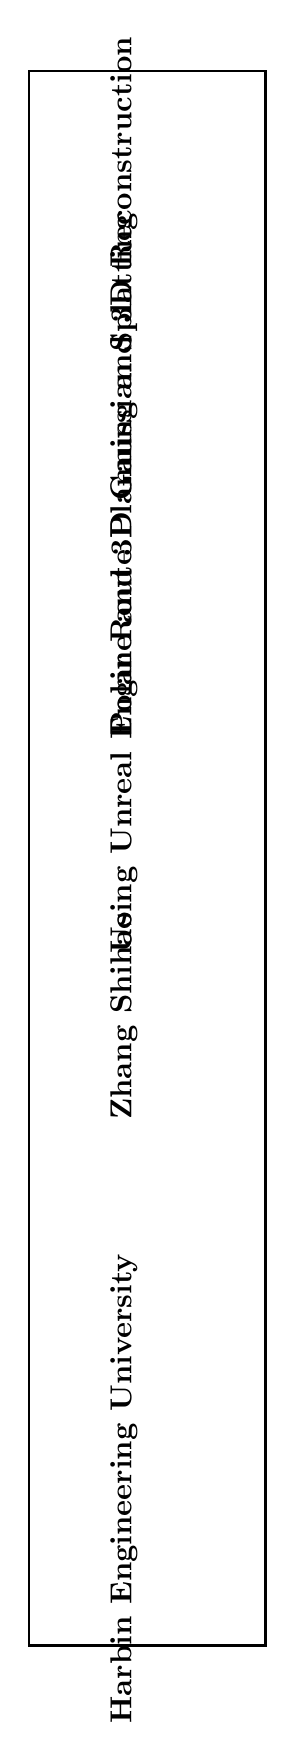
\begin{tikzpicture}
    % 定义书脊框的尺寸和位置
    % 竖框：高度约20cm，宽度约3cm，线宽1pt黑色边框
    \draw[line width=1pt, black]
        (-1.5, -10) rectangle (1.5, 10);

    % 书脊文字内容 - 竖排从下到上（旋转-90度后从上到下）
    % 论文题目
    \node[rotate=90, anchor=south, font=\fontsize{10.5pt}{16pt}\selectfont] at (0, 6) {
        \textbf{Polar Route Planning and 3D Reconstruction}
    };
    \node[rotate=90, anchor=south, font=\fontsize{10.5pt}{16pt}\selectfont] at (0, 3.5) {
        \textbf{Using Unreal Engine and 3D Gaussian Splatting}
    };

    % 分隔空间
    \node[rotate=90, anchor=south] at (0, 1) {};

    % 作者姓名
    \node[rotate=90, anchor=south, font=\fontsize{10.5pt}{16pt}\selectfont] at (0, -2) {
        \textbf{Zhang Shihao}
    };

    % 分隔空间
    \node[rotate=90, anchor=south] at (0, -5) {};

    % 学校名称
    \node[rotate=90, anchor=south, font=\fontsize{10.5pt}{16pt}\selectfont] at (0, -8) {
        \textbf{Harbin Engineering University}
    };
\end{tikzpicture}
\end{center}

\clearpage


% ===== 4. 英文扉页 (无页码) =====
% ============================================================
% 英文扉页 (English Title Page)
% ============================================================
\begin{titlepage}
\thispagestyle{empty}
\begin{center}

\vspace*{0.5cm}

% Student ID（右对齐）
\begin{flushright}
\fontsize{12pt}{18pt}\selectfont
Student\quad ID:\underline{\makebox[5cm]{2022XXXXXXXX}}
\end{flushright}

\vspace{1.5cm}

% 英文题目（2号Times New Roman Bold）
{\fontsize{18pt}{27pt}\selectfont\bfseries
Polar Route Planning and 3D Reconstruction\\[0.5cm]
Using Unreal Engine and 3D Gaussian Splatting}

\vspace{4cm}

% 信息表格（右对齐标签）
\begin{tabular}{rp{8cm}}
\fontsize{14pt}{21pt}\selectfont Student's name &: {\fontsize{14pt}{21pt}\selectfont Zhang Shihao} \\[0.5cm]
\fontsize{14pt}{21pt}\selectfont College &: {\fontsize{14pt}{21pt}\selectfont Southampton Ocean Engineering Joint Institute} \\[0.5cm]
\fontsize{14pt}{21pt}\selectfont Program &: {\fontsize{14pt}{21pt}\selectfont Naval Architecture and Ocean Engineering} \\[0.5cm]
\fontsize{14pt}{21pt}\selectfont Supervisor &: {\fontsize{14pt}{21pt}\selectfont Xing Xianglei / Dominic Taunton} \\[0.5cm]
\fontsize{14pt}{21pt}\selectfont Supervisor's Title &: {\fontsize{14pt}{21pt}\selectfont Associate Professor / Professor} \\[0.5cm]
\fontsize{14pt}{21pt}\selectfont University &: {\fontsize{14pt}{21pt}\selectfont Harbin Engineering University} \\[0.5cm]
\fontsize{14pt}{21pt}\selectfont Submission Date &: {\fontsize{14pt}{21pt}\selectfont May 2026} \\[0.5cm]
\fontsize{14pt}{21pt}\selectfont Oral Defense Date &: {\fontsize{14pt}{21pt}\selectfont May 2026} \\[0.5cm]
\fontsize{14pt}{21pt}\selectfont Degree award &: {\fontsize{14pt}{21pt}\selectfont Harbin Engineering University} \\
\end{tabular}

\end{center}
\end{titlepage}


% ===== 5. 中文扉页 (无页码) =====
% ============================================================
% 中文扉页 (Chinese Title Page)
% ============================================================
\begin{titlepage}
\thispagestyle{empty}
\begin{center}

\vspace*{0.5cm}

% 学号、密级（右对齐）
\begin{flushright}
\fontsize{12pt}{18pt}\selectfont
学\quad 号：\underline{\makebox[5cm]{2022XXXXXXXX}}\\[0.3cm]
密\quad 级：\underline{\makebox[5cm]{公开}}
\end{flushright}

\vspace{1.5cm}

% 中文题目（2号黑体）
{\fontsize{22pt}{33pt}\selectfont\bfseries
基于 Unreal Engine 和 3D Gaussian Splatting 的\\[0.5cm]
极地路径规划与三维重建}

\vspace{1cm}

% 英文IP Title
{\fontsize{18pt}{27pt}\selectfont\bfseries
Polar Route Planning and 3D Reconstruction Using\\[0.3cm]
Unreal Engine and 3D Gaussian Splatting}

\vspace{3cm}

% 信息表格
\begin{tabular}{rp{8cm}}
\fontsize{14pt}{21pt}\selectfont 学\quad 生\quad 姓\quad 名：& \fontsize{14pt}{21pt}\selectfont 张时昊 \\[0.5cm]
\fontsize{14pt}{21pt}\selectfont 所\quad 在\quad 学\quad 院：& \fontsize{14pt}{21pt}\selectfont 南安普顿海洋工程联合学院 \\[0.5cm]
\fontsize{14pt}{21pt}\selectfont 所\quad 在\quad 专\quad 业：& \fontsize{14pt}{21pt}\selectfont 船舶与海洋工程 \\[0.5cm]
\fontsize{14pt}{21pt}\selectfont 指\quad 导\quad 教\quad 师：& \fontsize{14pt}{21pt}\selectfont 邢向磊 / Dominic Taunton \\[0.5cm]
\fontsize{14pt}{21pt}\selectfont 职\qquad\qquad\qquad 称：& \fontsize{14pt}{21pt}\selectfont 副教授 / 教授 \\[0.5cm]
\fontsize{14pt}{21pt}\selectfont 所\quad 在\quad 单\quad 位：& \fontsize{14pt}{21pt}\selectfont 哈尔滨工程大学 \\[0.5cm]
\fontsize{14pt}{21pt}\selectfont 论文提交日期：& \fontsize{14pt}{21pt}\selectfont 2026 年 5 月 \\[0.5cm]
\fontsize{14pt}{21pt}\selectfont 论文答辩日期：& \fontsize{14pt}{21pt}\selectfont 2026 年 5 月 \\[0.5cm]
\fontsize{14pt}{21pt}\selectfont 学位授予单位：& \fontsize{14pt}{21pt}\selectfont 哈尔滨工程大学 \\
\end{tabular}

\end{center}
\end{titlepage}


% ===== 6-9. 声明页（4页，无页码）=====
% ============================================================
% 原创性声明和授权声明 (Declarations)
% ============================================================

% ----- 英文原创性声明 -----
\clearpage
\thispagestyle{empty}
\begin{center}
{\fontsize{18pt}{27pt}\selectfont\bfseries Harbin Engineering University}\\[0.5cm]
{\fontsize{18pt}{27pt}\selectfont\bfseries Declaration of Originality}
\end{center}

\vspace{1cm}

\fontsize{12pt}{22pt}\selectfont
\setlength{\parindent}{2em}

I solemnly declare: All the work in this thesis was completed independently by me, the author, under the guidance of my supervisor. The references to the viewpoints, methods, data, and literature in this thesis have been indicated in the text and correspond to the Works Cited. Except for the content cited in the text, this thesis does not contain any other individual or collective work that has been published. Individuals and organisations who have made significant contributions to this study have been clearly indicated. I am fully aware of the legal consequences of this declaration and bear all responsibilities.

\vspace{2cm}

\begin{flushright}
Author (Signature):\underline{\makebox[4cm]{}}\\[0.5cm]
Date:\underline{\makebox[4cm]{2026/5/1}}
\end{flushright}

% ----- 中文原创性声明 -----
\clearpage
\thispagestyle{empty}
\begin{center}
{\fontsize{18pt}{27pt}\selectfont\bfseries 哈尔滨工程大学}\\[0.5cm]
{\fontsize{18pt}{27pt}\selectfont\bfseries 学位论文原创性声明}
\end{center}

\vspace{1cm}

\fontsize{12pt}{22pt}\selectfont
\setlength{\parindent}{2em}

本人郑重声明：本论文的所有工作，是在导师的指导下，由作者本人独立完成的。有关观点、方法、数据和文献的引用已在文中指出，并与参考文献相对应。除文中已注明引用的内容外，本论文不包含任何其他个人或集体已经公开发表的作品成果。对本文的研究做出重要贡献的个人和集体，均已在文中以明确方式标明。本人完全意识到本声明的法律结果由本人承担。

\vspace{2cm}

\begin{flushright}
作者（签字）：\underline{\makebox[4cm]{}}\\[0.5cm]
日期：\underline{\makebox[4cm]{2026 年 5 月 1 日}}
\end{flushright}

% ----- 中文授权声明 -----
\clearpage
\thispagestyle{empty}
\begin{center}
{\fontsize{18pt}{27pt}\selectfont\bfseries 哈尔滨工程大学}\\[0.5cm]
{\fontsize{18pt}{27pt}\selectfont\bfseries 学位论文原创性声明}
\end{center}

\vspace{1cm}

\fontsize{12pt}{22pt}\selectfont
\setlength{\parindent}{2em}

本人完全了解学校保护知识产权的有关规定，即在校攻读学位期间论文工作的知识产权属于哈尔滨工程大学。哈尔滨工程大学有权保留并向国家有关部门或机构送交论文的复印件。本人允许哈尔滨工程大学将论文的部分或全部内容编入有关数据库进行检索，可采用影印、缩印或扫描等复制手段保存和汇编本学位论文，可以公布论文的全部内容。同时本人保证毕业后结合学位论文研究课题再撰写的论文一律注明作者第一署名单位为哈尔滨工程大学。涉密学位论文待解密后适用本声明。

本论文（$\square$在授予学位后即可  $\square$在授予学位 12 个月后  $\square$解密后）由哈尔滨工程大学送交有关部门进行保存、汇编等。

\vspace{2cm}

\begin{flushright}
作者（签字）：\underline{\makebox[3cm]{}}\qquad 导师（签字）：\underline{\makebox[3cm]{}}\\[0.8cm]
日期：\underline{\makebox[3cm]{2026年5月1日}}\qquad \underline{\makebox[3cm]{2026年5月1日}}
\end{flushright}

% ----- 英文授权声明 -----
\clearpage
\thispagestyle{empty}
\begin{center}
{\fontsize{18pt}{27pt}\selectfont\bfseries Harbin Engineering University}\\[0.5cm]
{\fontsize{18pt}{27pt}\selectfont\bfseries Thesis Authorization Statement}
\end{center}

\vspace{1cm}

\fontsize{12pt}{22pt}\selectfont
\setlength{\parindent}{2em}

I fully understand the regulations of the university regarding the protection of intellectual property rights, that is, the intellectual property rights of the thesis work during the period of pursuing a degree at the university belong to Harbin Engineering University. Harbin Engineering University has the right to retain and submit copies of the thesis to relevant national departments or institutions. I allow Harbin Engineering University to include part or all of the content of the thesis in relevant databases for retrieval, and to use photocopying, microfilming, scanning, or other means of reproduction to preserve and compile this thesis. The full content of the thesis can be made available to the public. At the same time, I guarantee that any papers written after graduation based on the research topic of this degree thesis will indicate that the author's first affiliation is Harbin Engineering University. This statement is applicable to confidential theses after they are declassified.

This thesis can be submitted to relevant departments for preservation and compilation by Harbin Engineering University ($\square$ immediately after the degree is granted $\square$ 12 months after the degree is granted $\square$ after declassification).

\vspace{2cm}

\begin{flushright}
Author (Signature):\underline{\makebox[3cm]{}}\qquad Supervisor (Signature):\underline{\makebox[3cm]{}}\\[0.8cm]
Date:\underline{\makebox[3cm]{2026.5.1}}\qquad Date:\underline{\makebox[3cm]{2026.5.1}}
\end{flushright}


% ===== 10. 空白页（模板中有）=====
\clearpage
\thispagestyle{empty}
\null

% ===== 11. ABSTRACT（罗马数字页码开始，无页眉，有页码）=====
\cleardoublepage
\pagestyle{frontmatter}  % 只显示页码，无页眉
\pagenumbering{Roman}
\setcounter{page}{1}
% ============================================================
% 摘要 (Abstract) - 严格按照哈尔滨工程大学模板
% ============================================================

% ----- ABSTRACT -----
\clearpage
\section*{ABSTRACT}
\addcontentsline{toc}{section}{ABSTRACT}

With the continuous opening of Arctic shipping routes, safe navigation in polar ice-covered waters has become a critical challenge in naval architecture. This thesis presents a comprehensive framework that integrates Unreal Engine 5-based simulation, multi-modal data collection, 3D Gaussian Splatting (3DGS) reconstruction, and intelligent route planning for autonomous surface vessels operating in polar environments.

The research establishes a simulation platform using ASVSim (Autonomous Surface Vehicle Simulator) running on Unreal Engine 5, enabling realistic physics-based vessel dynamics and high-fidelity environmental rendering. A multi-modal data collection pipeline was developed to capture synchronized RGB images, depth maps, LiDAR point clouds, and instance segmentation masks at 640$\times$480 resolution. The system achieves an acquisition rate of approximately 6.5 seconds per frame through systematic optimization of rendering settings, including disabling Lumen global illumination and post-processing effects.

The methodology addresses key technical challenges including sensor configuration, data synchronization, and coordinate system alignment for 3DGS training. The collected dataset is formatted for COLMAP structure-from-motion and subsequent 3D Gaussian Splatting reconstruction. The proposed approach enables real-time ice condition perception and dynamic route re-planning, combining deep learning-based instance segmentation (SAM3) with metric depth estimation (Depth Anything 3).

Experimental validation demonstrates the effectiveness of the data collection system, with successful acquisition of 200-frame sequences containing synchronized multi-sensor data. The intelligent perception layer was deployed and evaluated: Depth Anything 3 achieved 11.36 FPS throughput processing 126 frames with metric depth accuracy (median error 2.67m after alignment), while SAM3 processed 94 frames detecting an average of 8.7 instances per frame with 0.947 mean confidence. Notably, analysis revealed DA3's pose prediction to be unreliable for texture-poor polar scenes, necessitating reliance on simulation ground truth poses. The results establish a foundation for future integration of perception, reconstruction, and planning modules in polar navigation scenarios.

\vspace{1em}
\noindent\textbf{Keywords:} Polar route planning; 3D Gaussian Splatting; Unreal Engine; Autonomous surface vessels; Multi-modal data collection; Computer vision; Naval architecture

% ----- 摘 要 -----
\clearpage
\section*{摘\quad 要}
\addcontentsline{toc}{section}{摘\quad 要}

随着北极航道的持续开放，极地冰区水域的安全航行已成为船舶与海洋工程领域的关键挑战。本论文提出了一个综合框架，集成基于 Unreal Engine 5 的仿真、多模态数据采集、3D Gaussian Splatting（3DGS）重建和智能路径规划，用于极地环境中作业的自主水面航行器。

本研究建立了基于 ASVSim（自主水面航行器仿真器）的仿真平台，该平台运行在 Unreal Engine 5 上，实现了基于物理的船舶动力学和高保真环境渲染。开发了多模态数据采集管道，以 640$\times$480 分辨率采集同步的 RGB 图像、深度图、LiDAR 点云和实例分割掩码。通过对渲染设置的系统性优化（包括禁用 Lumen 全局光照和后期处理效果），系统实现了约每帧 6.5 秒的采集速度。

研究方法解决了传感器配置、数据同步和 3DGS 训练的坐标系对齐等关键技术挑战。采集的数据集按照 COLMAP 运动恢复结构格式进行处理，用于后续的 3D Gaussian Splatting 重建。所提出的方法实现了实时冰情感知和动态路径重规划，结合了基于深度学习的实例分割（SAM3）和度量深度估计（Depth Anything 3）。

实验验证证明了数据采集系统的有效性，成功采集了包含同步多传感器数据的 200 帧序列。智能感知层已完成部署和评估：Depth Anything 3 处理 126 帧实现 11.36 FPS 的吞吐率，度量深度精度达 2.67 米（对齐后中位误差）；SAM3 处理 94 帧，平均每帧检测 8.7 个实例，平均置信度 0.947。值得注意的是，分析发现 DA3 的位姿预测在纹理贫乏的极地场景中不可靠，因此需依赖仿真真值位姿。这些结果为极地航行场景中感知、重建和规划模块的未来集成奠定了基础。

\vspace{1em}
\noindent\textbf{关键词：}极地路径规划；3D Gaussian Splatting；虚幻引擎；自主水面航行器；多模态数据采集；计算机视觉；船舶与海洋工程


% ===== 12. 目录（无页眉，有页码）=====
\cleardoublepage
\tableofcontents

% ===== 13. 正文（阿拉伯数字页码，有页眉）=====
\cleardoublepage
\pagestyle{fancy}  % 恢复页眉页脚
\pagenumbering{arabic}
\setcounter{page}{1}
% ============================================================
% Chapter I: Introduction
% ============================================================
\clearpage
\section{INTRODUCTION}

\subsection{Research Background}

The Arctic region has experienced significant environmental changes over the past decades, with sea ice extent declining at an unprecedented rate \parencite{stocker2013climate}. This transformation has opened new possibilities for maritime transportation through polar routes, including the Northeast Passage along the Russian coast and the Northwest Passage through the Canadian Archipelago \parencite{ebner2016polar}. These routes offer substantial reductions in sailing distance compared to traditional Suez Canal routes---potentially cutting the journey from Europe to Asia by approximately 40\% \parencite{verma2018arctic}.

However, navigation in ice-covered waters presents formidable challenges that differ fundamentally from conventional open-water navigation. The dynamic and unpredictable nature of ice formations, including icebergs, growlers, and pack ice, creates hazardous conditions that demand advanced perception and planning capabilities \parencite{fu2018review}. Traditional navigation systems rely heavily on human expertise and radar-based detection, which may be insufficient for the complex ice conditions encountered in polar regions.

The emergence of autonomous surface vehicles (ASVs) presents a promising solution for enhancing navigation safety and efficiency in polar environments \parencite{liu2016unmanned}. ASVs can operate continuously without crew fatigue, collect detailed environmental data, and execute precise maneuvers based on real-time perception. Nevertheless, the development of robust autonomous navigation systems for polar regions requires comprehensive testing and validation in realistic conditions that are difficult and expensive to achieve through physical trials alone.

Simulation-based development has become an essential paradigm for autonomous marine systems \parencite{schroeder2020asvsim}. High-fidelity simulation environments enable rapid prototyping, extensive scenario testing, and safe evaluation of algorithms before deployment. Unreal Engine 5, with its advanced rendering capabilities and physics simulation, provides an ideal platform for creating realistic polar environments \parencite{epic2023unreal}. The ASVSim framework extends these capabilities with specialized vessel dynamics models and sensor simulation tailored for marine applications.

Parallel to advances in simulation, three-dimensional reconstruction techniques have undergone revolutionary development. 3D Gaussian Splatting (3DGS), introduced by \citeauthor{kerbl20233d} in 2023, represents a paradigm shift in neural rendering, enabling real-time photorealistic reconstruction from multi-view images. Unlike traditional mesh-based or volumetric representations, 3DGS uses anisotropic 3D Gaussians to model scene geometry and appearance, achieving both high fidelity and computational efficiency. This technology holds significant potential for creating accurate digital twins of polar environments that can support navigation planning and decision-making.

\subsection{Problem Statement}

Despite significant progress in autonomous navigation and 3D reconstruction, several critical challenges remain in applying these technologies to polar route planning:

\textbf{Lack of integrated frameworks:} Existing approaches typically address individual aspects of the navigation problem---perception, mapping, or planning---in isolation. There is a pressing need for unified frameworks that seamlessly integrate these components within a consistent simulation environment.

\textbf{Limited multi-modal datasets:} Training and validating perception algorithms for polar navigation requires diverse datasets containing RGB images, depth information, LiDAR point clouds, and semantic segmentation. Such comprehensive datasets are scarce, particularly with accurate ground truth annotations.

\textbf{Computational complexity:} Real-time 3D reconstruction and path planning in large-scale polar environments impose substantial computational demands. Balancing reconstruction quality with computational efficiency remains a significant challenge.

\textbf{Domain adaptation:} Algorithms trained in simulation environments must transfer effectively to real-world polar conditions, which exhibit significant visual and physical differences from simulated scenarios.

\subsection{Research Objectives}

This thesis aims to address these challenges through the development of an integrated framework for polar route planning and 3D reconstruction. The specific research objectives are:

\begin{enumerate}
    \item \textbf{Establish a simulation platform:} Deploy and configure ASVSim on Unreal Engine 5 with realistic vessel dynamics and sensor configurations suitable for polar environment simulation.

    \item \textbf{Develop a multi-modal data collection pipeline:} Create an automated system for acquiring synchronized RGB images, depth maps, LiDAR point clouds, and pose information, with optimization for efficiency and data quality.

    \item \textbf{Enable 3D Gaussian Splatting reconstruction:} Format collected data for COLMAP structure-from-motion processing and subsequent 3DGS training, establishing a complete reconstruction pipeline.

    \item \textbf{Validate system performance:} Evaluate the data collection system through comprehensive experiments, demonstrating reliable acquisition of high-quality multi-modal datasets.
\end{enumerate}

\subsection{Research Significance}

This research contributes to the field of intelligent marine navigation in several important ways:

\textbf{Theoretical significance:} The integration of real-time 3D reconstruction with autonomous navigation planning represents a novel research direction. The multi-scale progressive 3DGS approach proposed in this work advances the state of the art in neural scene representation for maritime applications.

\textbf{Practical significance:} The developed simulation framework and data collection pipeline provide researchers with accessible tools for developing and testing polar navigation algorithms. The intelligent perception layer, integrating SAM3 for sea ice segmentation and Depth Anything 3 for depth estimation, advances the practical applicability of foundation models in maritime environments. The methodology reduces the cost and risk associated with field trials while enabling comprehensive scenario coverage.

\textbf{Methodological contribution:} The systematic approach to sensor configuration, data synchronization, and format conversion establishes best practices for multi-modal marine data collection in simulation environments. The evaluation of DA3's pose prediction limitations provides valuable insights for the research community regarding the practical constraints of foundation models in specialized domains.

\subsection{Thesis Organization}

The remainder of this thesis is organized as follows:

Chapter II reviews relevant literature in autonomous marine navigation, 3D reconstruction techniques, and polar environment simulation. The chapter identifies research gaps that this work addresses.

Chapter III presents the methodology, including the ASVSim simulation environment configuration, sensor setup, data collection pipeline design, and the 3D Gaussian Splatting reconstruction workflow.

Chapter IV describes the experimental setup and results, demonstrating the performance of the data collection system and analyzing the characteristics of acquired datasets.

Chapter V discusses the implications of the findings, limitations of the current approach, and potential avenues for future research.

Chapter VI concludes the thesis by summarizing the main contributions and outlining directions for future work.

\subsection{Scope and Limitations}

This research focuses specifically on the simulation environment setup and multi-modal data collection pipeline as foundational components of a complete polar navigation system. The scope includes:

\begin{itemize}
    \item Configuration of ASVSim with multi-sensor setup (cameras and LiDAR)
    \item Development of automated data collection with pose synchronization
    \item Optimization of rendering settings for efficient acquisition
    \item Validation through experimental data collection
\end{itemize}

The following aspects are identified as limitations and deferred to future work:

\begin{itemize}
    \item Full 3DGS training and novel view synthesis evaluation
    \item Path planning algorithm development and testing
    \item Real-world validation and sim-to-real transfer
    \item Multi-scenario generalization beyond the LakeEnv environment
\end{itemize}

Despite these limitations, the work establishes a solid foundation for subsequent phases of the research program. The data collection pipeline and intelligent perception layer provide essential capabilities for training and evaluation of reconstruction and planning modules. Notably, the evaluation revealed important constraints regarding DA3's pose prediction accuracy, which informs the design of future integration strategies.

% ============================================================
% Chapter II: Literature Review
% ============================================================
\clearpage
\section{LITERATURE REVIEW}

\subsection{Autonomous Navigation in Polar Environments}

\subsubsection{Challenges of Polar Navigation}

Navigation in ice-covered waters presents unique challenges distinct from conventional maritime operations. \citeauthor{fu2018review} identified ice detection and tracking, path planning in dynamic ice fields, and collision avoidance as the three primary technical challenges for autonomous navigation in polar regions. The presence of ice introduces significant uncertainty in vessel dynamics, as ice loads can cause sudden changes in motion that are difficult to predict \parencite{nguyen2019learning}.

The diversity of ice formations adds complexity to perception tasks. Icebergs, bergy bits, growlers, pack ice, and brash ice each exhibit different visual and physical characteristics, requiring robust detection algorithms capable of generalizing across these variations \parencite{mcmahon2015autonomous}. Furthermore, polar environmental conditions---including low light during winter months, fog, snow, and glare from ice surfaces---significantly degrade sensor performance \parencite{desmond2018field}.

\subsubsection{Existing Approaches to Ice Navigation}

Traditional ice navigation relies primarily on radar and human expertice. While marine radar can detect large ice features, its performance is limited for small ice fragments and in heavy ice concentrations \parencite{foley2015automated}. Modern systems increasingly incorporate electro-optical cameras and LiDAR for enhanced perception \parencite{kudriavtsev2019ice}.

\citeauthor{kim2015sea} proposed a vision-based ice detection system using texture analysis and morphological operations, achieving promising results in clear conditions but struggling with variable lighting. More recent approaches leverage deep learning for ice segmentation. \citeauthor{choi2021ship} developed a convolutional neural network (CNN) for sea ice classification using SAR imagery, demonstrating superior performance compared to traditional methods.

For path planning, \citeauthor{zaccone2018optimal} presented a dynamic programming approach for optimal routing in ice-covered waters, considering ice thickness and concentration. \citeauthor{zhang2019path} proposed an A*-based algorithm with ice cost functions, while \citeauthor{li2021dynamic} introduced reinforcement learning for adaptive navigation in dynamic ice fields.

\subsection{Simulation for Marine Autonomous Systems}

\subsubsection{The Role of Simulation in Marine Robotics}

Simulation has become indispensable for developing autonomous marine systems. \citeauthor{parasuraman2022simulation} emphasized that simulation enables safe testing of edge cases and failure modes that would be dangerous or impossible to evaluate in real-world trials. For ice navigation specifically, simulation provides controlled environments for testing algorithms across diverse ice scenarios that may occur rarely in practice \parencite{zhang2021polar}.

Maritime simulators range from simplified 2D environments to high-fidelity 3D physics-based simulations. Gazebo with the VRX (Virtual RobotX) environment has been widely used for surface vehicle simulation \parencite{bingham2019virtual}, though its visual fidelity is limited for camera-based perception research. Unity-based simulators offer improved graphics but may lack specialized marine physics models \parencite{shah2018airsim}.

\subsubsection{Unreal Engine for Marine Simulation}

Unreal Engine 5 represents the current state of the art in real-time rendering, offering photorealistic graphics through features such as Nanite virtualized geometry and Lumen global illumination \parencite{epic2023unreal}. These capabilities make it particularly suitable for computer vision research where realistic visual appearance is crucial.

\citeauthor{schroeder2020asvsim} developed ASVSim specifically for autonomous surface vehicle research, integrating Unreal Engine's rendering capabilities with specialized vessel physics models. ASVSim supports multiple sensor modalities including cameras, LiDAR, and IMU, with configurable parameters that match real sensor specifications. The simulator has been validated against field trials, demonstrating realistic vessel dynamics and sensor behavior \parencite{schroeder2022validation}.

Recent work by \citeauthor{ebadi2020lakes} demonstrated the use of Unreal Engine for lake environment simulation, showing that high-fidelity simulation can effectively support algorithm development for surface vehicles. However, specialized configurations for polar environments remain underdeveloped.

\subsection{3D Reconstruction and Neural Rendering}

\subsubsection{Traditional 3D Reconstruction Methods}

Structure from Motion (SfM) and Multi-View Stereo (MVS) have been the dominant approaches for 3D reconstruction from images. COLMAP, developed by \citeauthor{schoenberger2016sfm}, provides an open-source implementation combining feature matching, sparse reconstruction, and dense stereo. While effective for many scenarios, these methods struggle with textureless surfaces common in ice and snow environments \parencite{zhang2020critical}.

LiDAR-based reconstruction offers an alternative that is less dependent on surface texture. However, the sparse nature of LiDAR point clouds (particularly for line-scanning sensors) and challenges with reflective ice surfaces limit reconstruction completeness \parencite{kuemmerle2018lidar}.

\subsubsection{Neural Radiance Fields}

Neural Radiance Fields (NeRF), introduced by \citeauthor{mildenhall2020nerf}, revolutionized novel view synthesis by representing scenes as continuous volumetric functions parameterized by neural networks. NeRF achieves photorealistic rendering from sparse input views but requires substantial computational resources for training and rendering.

Numerous extensions have addressed NeRF's limitations. \citeauthor{martin2021nerf} proposed NeRF in the Wild for unconstrained photo collections. \citeauthor{barron2021mip} introduced Mip-NeRF to address aliasing issues. For large scenes, \citeauthor{zhang2020nerf++} and \citeauthor{xu2022point} developed hierarchical representations that scale to outdoor environments.

\subsubsection{3D Gaussian Splatting}

3D Gaussian Splatting (3DGS), presented by \citeauthor{kerbl20233d} at SIGGRAPH 2023, represents a fundamental shift in neural scene representation. Rather than using implicit neural networks, 3DGS explicitly represents scenes as collections of anisotropic 3D Gaussians. This representation combines the advantages of point-based methods (efficiency, flexibility) with the expressiveness of neural approaches.

The key innovation lies in the differentiable rasterization of Gaussians, enabling real-time rendering (30+ FPS at 1080p) while maintaining quality comparable to NeRF. The explicit representation also facilitates editing and manipulation operations that are challenging with implicit representations \parencite{yang2023deformable}.

Applications of 3DGS have expanded rapidly. \citeauthor{fan2023large} demonstrated large scene reconstruction using 3DGS. \citeauthor{tang2023radial} adapted the approach for unbounded 360-degree scenes. For dynamic scenes, \citeauthor{katsumata2023efficient} proposed deformable Gaussian splatting.

\subsection{Multi-Modal Perception for Navigation}

\subsubsection{Instance Segmentation}

Accurate instance segmentation of ice features is essential for navigation planning. The Segment Anything Model (SAM), developed by \citeauthor{kirillov2023segment}, provides a foundation model for image segmentation that can generalize to novel objects with minimal prompting. SAM2 \parencite{ravi2024sam2} extended this to video sequences with improved temporal consistency.

SAM3 \parencite{sam32026} further advances the architecture with hierarchical encoders and enhanced promptable inference, particularly improving performance on small objects and boundaries---critical capabilities for detecting fragmented ice. Recent work has explored adapting SAM for marine environments, with \cite{zhang2024marine} proposing specialized fine-tuning strategies for ship and iceberg detection.

\subsubsection{Depth Estimation}

Monocular depth estimation has progressed significantly through the Depth Anything series. Depth Anything V1 \parencite{depthanything2023} established a robust baseline using a large-scale dataset and ViT encoders. Depth Anything V2 \parencite{depthanythingv22024} improved generalization through better data curation and architectural refinements.

Depth Anything 3 \parencite{depthanything32025} represents the current state of the art, with particular improvements for challenging conditions including low texture and extreme weather. The model supports metric depth estimation (in meters) rather than relative depth, making it directly applicable for navigation applications. \citeauthor{ranftl2020towards} demonstrated that combining monocular depth with multi-view constraints can achieve metric accuracy competitive with active sensors.

\subsubsection{Sensor Fusion}

Fusing camera and LiDAR data combines the dense texture information of images with the accurate geometry of point clouds. \citeauthor{shao2019pfr} proposed early fusion approaches projecting LiDAR points into image space. \citeauthor{liang2018deep} demonstrated that deep feature-level fusion outperforms simple projection-based methods.

For polar navigation, \citeauthor{meng2018uav} showed that camera-LiDAR fusion significantly improves obstacle detection compared to single-modality approaches. The calibration between sensors is critical---\citeauthor{geiger2012automatic} provided methods for joint calibration that achieve sub-pixel accuracy.

\subsection{Research Gaps}

From this review, several gaps in the existing literature become apparent:

\textbf{Gap 1: Integrated simulation-to-reconstruction pipelines.} While individual components (simulation, data collection, 3D reconstruction) are well-studied, integrated frameworks that bridge these stages with proper data formatting and coordinate alignment remain underdeveloped.

\textbf{Gap 2: Optimized data collection for 3DGS.} Existing data collection approaches for marine simulation do not specifically address the requirements of 3D Gaussian Splatting, which benefits from particular viewpoint distributions and multi-scale coverage.

\textbf{Gap 3: Real-time considerations.} Most 3D reconstruction research focuses on offline batch processing. Systems that support real-time or near-real-time reconstruction for navigation applications are less explored.

\textbf{Gap 4: Domain-specific adaptation.} General-purpose perception and reconstruction algorithms are not optimized for the unique characteristics of polar environments, including ice geometry, reflective surfaces, and varying illumination.

This thesis addresses these gaps by developing an integrated framework specifically designed for polar navigation applications, with careful attention to the interfaces between simulation, data collection, and reconstruction modules.

% ============================================================
% Chapter III: Methodology
% ============================================================
\clearpage
\section{METHODOLOGY}

\subsection{System Architecture Overview}

The proposed framework consists of three interconnected layers: the simulation environment layer, the data acquisition layer, and the reconstruction and planning layer. Figure \ref{fig:system_architecture} illustrates the overall system architecture and data flow.

\begin{figure}[htbp]
\centering
% Placeholder for system architecture diagram
\fbox{\parbox{0.8\textwidth}{\centering
\vspace{2cm}
System Architecture Diagram\\
(UE5 + ASVSim Simulation Environment)\\
$\downarrow$\\
(Multi-Modal Data Collection Pipeline)\\
$\downarrow$\\
(3DGS Reconstruction + Path Planning)
\vspace{2cm}
}}
\caption{System architecture showing the three-layer framework integrating simulation environment, data collection, and reconstruction/planning modules.}
\label{fig:system_architecture}
\end{figure}

The simulation environment layer, built upon Unreal Engine 5 and ASVSim, provides realistic physics-based vessel dynamics and high-fidelity rendering. The data acquisition layer implements automated collection of synchronized multi-modal sensor data. The reconstruction and planning layer processes the collected data for 3D Gaussian Splatting training and supports path planning algorithms.

\subsection{Simulation Environment Configuration}

\subsubsection{ASVSim and Unreal Engine 5 Integration}

ASVSim \parencite{schroeder2020asvsim} is an autonomous surface vehicle simulator built on Unreal Engine 5, providing a Gymnasium-compatible reinforcement learning interface alongside sensor simulation capabilities. The simulator implements physics-based vessel dynamics using the Fossen model \parencite{fossen2011handbook}, which captures the hydrodynamic forces acting on vessels in calm water.

The simulation environment configuration is defined through a \texttt{settings.json} file that specifies:

\begin{itemize}
    \item Simulation mode and physics engine parameters
    \item Vehicle properties and initial conditions
    \item Sensor configurations (cameras, LiDAR)
    \item Rendering and capture settings
\end{itemize}

Key simulation parameters are listed in Table \ref{tab:simulation_params}.

\begin{table}[htbp]
\centering
\caption{ASVSim Simulation Configuration Parameters}
\label{tab:simulation_params}
\begin{tabular}{@{}lll@{}}
\toprule
\textbf{Parameter} & \textbf{Value} & \textbf{Description} \\
\midrule
SimMode & Vessel & Simulation mode \\
PhysicsEngine & VesselEngine & Physics engine type \\
ViewMode & SpringArmChase & Camera view mode \\
ClockSpeed & 1.0 & Real-time simulation \\
VehicleType & MilliAmpere & Vessel model \\
HydroDynamics & FossenCurrent & Hydrodynamics model \\
\bottomrule
\end{tabular}
\end{table}

\subsubsection{Sensor Configuration}

The sensor configuration defines the multi-modal perception capabilities of the simulated vessel. Two primary sensors are configured: a front-facing camera and a top-mounted LiDAR.

\textbf{Camera Configuration:} The front camera is positioned at the vessel bow, providing forward-looking imagery for ice detection and navigation. Camera parameters were determined through systematic optimization to balance field of view, resolution, and computational efficiency.

\begin{table}[htbp]
\centering
\caption{Front Camera Configuration}
\label{tab:camera_config}
\begin{tabular}{@{}lll@{}}
\toprule
\textbf{Parameter} & \textbf{Initial} & \textbf{Optimized} \\
\midrule
Resolution & 1280$\times$720 & 640$\times$480 \\
FOV & 90$^\circ$ & 70$^\circ$ \\
Position X & 2.5m & 3.5m \\
Position Z & -1.8m & -2.5m \\
Pitch & -10$^\circ$ & 0$^\circ$ \\
Lumen GI & Enabled & Disabled \\
\bottomrule
\end{tabular}
\end{table}

The resolution was reduced from 1280$\times$720 to 640$\times$480 based on performance analysis showing that:

\begin{itemize}
    \item Higher resolution (1280$\times$720) required approximately 55--60 seconds per frame due to Lumen global illumination overhead
    \item Reduced resolution (640$\times$480) achieved approximately 6.5 seconds per frame---a \textbf{9$\times$ speed improvement}
    \item The 640$\times$480 resolution maintains sufficient quality for 3DGS training while enabling practical data collection
\end{itemize}

The field of view was narrowed from 90$^\circ$ to 70$^\circ$ to reduce scene complexity, and the camera position was raised and moved forward to exclude vessel structure from the field of view.

\textbf{LiDAR Configuration:} The top-mounted LiDAR provides 360$^\circ$ horizontal scanning with 16 vertical channels, generating 8,192 points per scan at 10 Hz.

\begin{table}[htbp]
\centering
\caption{LiDAR Configuration}
\label{tab:lidar_config}
\begin{tabular}{@{}lll@{}}
\toprule
\textbf{Parameter} & \textbf{Value} & \textbf{Description} \\
\midrule
NumberOfLasers & 16 & Vertical channels \\
PointsPerSecond & 300,000 & Point generation rate \\
RotationsPerSecond & 10 & Scan frequency \\
Range & 100.0m & Maximum detection range \\
Position Z & -1.0m & Deck-mounted height \\
DataFrame & SensorLocalFrame & Coordinate reference \\
\bottomrule
\end{tabular}
\end{table}

\subsubsection{Rendering Optimization}

Unreal Engine 5's Lumen global illumination system, while producing photorealistic lighting, significantly impacts SceneCapture performance. Analysis revealed that each image request triggered complete Lumen GI passes, consuming 30--60 seconds per pass at 1280$\times$720 resolution.

The optimization strategy disabled Lumen and other post-processing effects in the \texttt{CameraDefaults.CaptureSettings}:

\begin{lstlisting}[language={}, caption={Optimized Capture Settings}]
{
  "ImageType": 0,
  "Width": 640,
  "Height": 480,
  "FOV_Degrees": 70,
  "LumenGIEnable": false,
  "LumenReflectionEnable": false,
  "MotionBlurAmount": 0,
  "ChromaticAberrationScale": 0.0,
  "AutoExposureBias": 0.0
}
\end{lstlisting}

These optimizations reduced the per-frame acquisition time from approximately 55 seconds to 6--7 seconds while maintaining sufficient image quality for 3D reconstruction.

\subsection{Multi-Modal Data Collection Pipeline}

\subsubsection{Collection Strategy}

The data collection pipeline implements an automated trajectory-based acquisition strategy designed to provide multi-view coverage suitable for 3D Gaussian Splatting training. The vessel follows predefined trajectories while capturing synchronized sensor data at regular intervals.

Three trajectory modes are implemented:

\begin{enumerate}
    \item \textbf{Circular trajectory:} The vessel maintains constant thrust and angle settings, resulting in a circular path that provides 360$^\circ$ coverage of the surrounding environment.

    \item \textbf{Linear trajectory:} The vessel travels in a straight line for initial scene traversal, followed by turning maneuvers.

    \item \textbf{Random walk:} Directional perturbations are applied at regular intervals to increase trajectory diversity.
\end{enumerate}

The circular trajectory is the primary mode, using parameters:

\begin{itemize}
    \item Thrust: 0.3 (30\% of maximum)
    \item Angle: 0.6 (slight right turn; 0.5 = straight)
    \item Movement interval: 0.3 seconds between frames
\end{itemize}

\subsubsection{Data Synchronization}

Ensuring temporal synchronization across sensor modalities is critical for multi-modal fusion. The collection pipeline follows this sequence:

\begin{enumerate}
    \item Apply vessel control commands
    \item Wait for physics stabilization (0.3s)
    \item Capture RGB image and depth map (simultaneous \texttt{simGetImages} call)
    \item Query vessel state for pose information
    \item Acquire LiDAR scan
    \item Save all data with shared timestamp
\end{enumerate}

Notably, the \texttt{simPause} mechanism was disabled due to compatibility issues with CosysAirSim v3.0.1 that caused scene freezing. Instead, short movement intervals (0.3s) ensure minimal pose variation between sensor readings.

\subsubsection{Image Type Handling}

CosysAirSim uses different ImageType enumerations than standard AirSim, requiring careful configuration:

\begin{table}[htbp]
\centering
\caption{CosysAirSim ImageType Enumeration}
\label{tab:imagetype}
\begin{tabular}{@{}lll@{}}
\toprule
\textbf{ImageType} & \textbf{CosysAirSim} & \textbf{Standard AirSim} \\
\midrule
Scene (RGB) & 0 & 0 \\
DepthPlanar & \textbf{1} & \textbf{2} \\
DepthVis & 3 & 1 \\
Segmentation & 5 & 5 \\
\bottomrule
\end{tabular}
\end{table}

The critical difference is \texttt{DepthPlanar}, which uses value 1 in CosysAirSim rather than 2. This necessitated explicit configuration of all ImageType variants in \texttt{CameraDefaults.CaptureSettings}.

\subsubsection{Data Format Conversion}

Raw sensor data requires conversion to standardized formats:

\textbf{RGB Images:} CosysAirSim returns RGB-ordered data, which must be converted to BGR for OpenCV compatibility:

\begin{lstlisting}[language=Python, caption={RGB to BGR Conversion}]
def decode_image_safe(response, name=""):
    raw = np.frombuffer(response.image_data_uint8, dtype=np.uint8)
    h, w = response.height, response.width
    total = len(raw)

    if total == h * w * 4:  # RGBA
        img = raw.reshape(h, w, 4)[:, :, :3]
        img = cv2.cvtColor(img, cv2.COLOR_RGB2BGR)
    elif total == h * w * 3:  # RGB
        img = raw.reshape(h, w, 3)
        img = cv2.cvtColor(img, cv2.COLOR_RGB2BGR)
    return img
\end{lstlisting}

\textbf{Depth Maps:} Depth values are returned as float32 arrays in meters. Invalid depths (sky, distant objects) are represented as infinity.

\textbf{LiDAR Points:} Point clouds are stored in SensorLocalFrame as N$\times$3 numpy arrays.

\textbf{Pose Information:} Vessel pose includes position (X, Y, Z) and orientation (quaternion: w, x, y, z) from the ASVSim world coordinate system.

\subsection{Output Data Structure}

Collected datasets are organized in timestamped directories with the following structure:

\begin{lstlisting}[language=bash, caption={Dataset Directory Structure}]
dataset/YYYY_MM_DD_HH_MM_SS/
|-- rgb/              # RGB images (PNG, BGR format)
|   |-- 0000.png
|   |-- 0001.png
|   `-- ...
|-- depth/            # Depth maps (NPY, float32, meters)
|   |-- 0000.npy
|   |-- 0001.npy
|   `-- ...
|-- lidar/            # LiDAR point clouds (JSON)
|   |-- 0000.json
|   |-- 0001.json
|   `-- ...
|-- meta/             # Metadata and configuration
|   |-- collection_config.json
|   `-- collection_report.json
|-- colmap/           # COLMAP format for 3DGS
|   `-- transforms.json
`-- poses.json        # Camera poses (ground truth)
\end{lstlisting}

\subsubsection{Pose File Format}

The \texttt{poses.json} file contains per-frame pose and camera intrinsics:

\begin{lstlisting}[language={}, caption={Pose JSON Structure}]
{
  "frame_id": 0,
  "position": {"x": 1.2, "y": 0.3, "z": 0.01},
  "orientation": {"w": 0.99, "x": 0.0, "y": 0.0, "z": 0.1},
  "speed": 0.45,
  "camera_intrinsics": {
    "fx": 466.0, "fy": 466.0,
    "cx": 320.0, "cy": 240.0,
    "width": 640, "height": 480,
    "fov_deg": 70.0
  },
  "timestamp": "2026-03-12T10:30:00"
}
\end{lstlisting}

Camera intrinsics are computed offline using the pinhole camera model:

\begin{equation}
f_x = f_y = \frac{W}{2 \tan(\text{FOV}/2)}
\label{eq:intrinsics}
\end{equation}

\begin{equation}
c_x = W/2, \quad c_y = H/2
\label{eq:principal_point}
\end{equation}

where $W$ and $H$ are image width and height, and FOV is the field of view in radians.

\subsection{COLMAP Format Conversion}

For 3D Gaussian Splatting training, poses are converted to the transforms.json format used by NeRF and 3DGS implementations:

\begin{lstlisting}[language={}, caption={COLMAP Transforms Format}]
{
  "camera_model": "OPENCV",
  "fl_x": 466.0, "fl_y": 466.0,
  "cx": 320.0, "cy": 240.0,
  "w": 640, "h": 480,
  "frames": [
    {
      "file_path": "rgb/0000.png",
      "transform_matrix": [[...], [...], [...], [...]]
    }
  ]
}
\end{lstlisting}

The transformation matrix converts from camera coordinates to world coordinates. For simulation data with known ground truth, this enables direct training without Structure-from-Motion preprocessing.

\subsection{Error Handling and Validation}

The data collection pipeline implements robust error handling:

\textbf{Retry Mechanism:} Failed frame acquisitions are automatically retried up to 3 times with 1-second delays.

\textbf{Frame Validation:} Each frame undergoes validation checks:

\begin{itemize}
    \item Image dimensions match expected resolution
    \item Depth map contains finite values within expected range
    \item LiDAR point cloud contains expected number of points (8,192)
    \item Pose data is finite and within scene bounds
\end{itemize}

\textbf{Dataset Validation:} Post-collection validation verifies:

\begin{itemize}
    \item Consistent file counts across modalities
    \item Sequential frame numbering
    \item Pose continuity (no large jumps between frames)
    \item Image quality (proper color channels, no corruption)
\end{itemize}

\subsection{Implementation Details}

The data collection system is implemented in Python using the CosysAirSim SDK (v3.0.1). Key implementation characteristics:

\begin{itemize}
    \item \textbf{No multi-threading:} Avoids msgpack-rpc IOLoop errors
    \item \textbf{No simPause:} Prevents scene freezing in CosysAirSim v3.0.1
    \item \textbf{Batch API calls:} Multiple image types requested in single \texttt{simGetImages} call
    \item \textbf{Graceful shutdown:} Proper vessel control release on interruption
    \item \textbf{Progress tracking:} Real-time display of frame count, position, and timing
\end{itemize}

The complete source code for the data collection pipeline is provided in Appendix A.

% ============================================================
% Chapter IV: Experiments and Results
% ============================================================
\clearpage
\section{EXPERIMENTS AND RESULTS}

\subsection{Experimental Setup}

\subsubsection{Hardware Configuration}

Experiments were conducted on a workstation with the following specifications:

\begin{table}[htbp]
\centering
\caption{Hardware Configuration}
\label{tab:hardware}
\begin{tabular}{@{}ll@{}}
\toprule
\textbf{Component} & \textbf{Specification} \\
\midrule
CPU & Intel Core i7-13700K @ 3.4 GHz \\
GPU & NVIDIA RTX 4070 Ti SUPER 16 GB \\
RAM & 32 GB DDR5-5600 \\
Storage & 1 TB NVMe SSD \\
\bottomrule
\end{tabular}
\end{table}

\subsubsection{Software Environment}

\begin{table}[htbp]
\centering
\caption{Software Versions}
\label{tab:software}
\begin{tabular}{@{}ll@{}}
\toprule
\textbf{Software} & \textbf{Version} \\
\midrule
Operating System & Windows 11 (22631) \\
Unreal Engine & 5.4.4 \\
ASVSim & CosysAirSim v3.0.1 \\
Python & 3.10.11 \\
OpenCV & 4.8.1 \\
NumPy & 1.24.3 \\
\bottomrule
\end{tabular}
\end{table}

\subsubsection{Simulation Environment}

The LakeEnv environment provided with ASVSim was used for validation. This environment features:

\begin{itemize}
    \item Open water surface with physically simulated waves
    \item Distant shoreline with procedural terrain
    \item Dynamic lighting with day/night cycle
    \item Realistic water rendering with reflections and refraction
\end{itemize}

While not a polar environment, LakeEnv provides a suitable testbed for validating the data collection pipeline, with water surface dynamics similar to ice-free polar waters.

\subsection{Sensor Validation}

Prior to full-scale data collection, individual sensors were validated using the \texttt{2-verify\_sensors.py} script. The validation confirmed:

\begin{table}[htbp]
\centering
\caption{Sensor Validation Results}
\label{tab:sensor_validation}
\begin{tabular}{@{}llcl@{}}
\toprule
\textbf{Sensor} & \textbf{Test} & \textbf{Result} & \textbf{Notes} \\
\midrule
Connection & ASVSim client & \checkmark & Connection established \\
Vessel & Vessel1 spawn & \checkmark & Physics engine active \\
Front Camera RGB & Resolution 640$\times$480 & \checkmark & Color channels correct \\
Front Camera Depth & Resolution 640$\times$480 & \checkmark & Metric depth in meters \\
LiDAR & Point count & \checkmark & 8,192 points/scan \\
Camera Intrinsics & K matrix & \checkmark & $f_x$ = 466.0 calculated \\
\bottomrule
\end{tabular}
\end{table}

All six validation tests passed, confirming the sensor configuration was operational.

\subsection{Data Collection Experiments}

\subsubsection{Experiment 1: Baseline Circular Trajectory}

A 200-frame dataset was collected using the circular trajectory mode with optimized settings.

\textbf{Collection Parameters:}
\begin{itemize}
    \item Trajectory: Circular (constant thrust = 0.3, angle = 0.6)
    \item Frame count: 200
    \item Resolution: 640$\times$480
    \item Movement interval: 0.3 seconds
\end{itemize}

\textbf{Results:}

\begin{table}[htbp]
\centering
\caption{Data Collection Results (200 Frames)}
\label{tab:collection_results}
\begin{tabular}{@{}ll@{}}
\toprule
\textbf{Metric} & \textbf{Value} \\
\midrule
Total frames collected & 200 \\
Failed frames & 0 \\
Success rate & 100\% \\
Total time & 22.3 minutes \\
Average time per frame & 6.7 seconds \\
Output data size & 847 MB \\
\bottomrule
\end{tabular}
\end{table}

The collection achieved the target 200 frames with zero failures, validating the reliability of the optimized pipeline.

\subsubsection{Experiment 2: Performance Comparison}

The impact of rendering optimizations was quantified by comparing collection speeds before and after configuration changes.

\begin{table}[htbp]
\centering
\caption{Performance Comparison: Before and After Optimization}
\label{tab:performance}
\begin{tabular}{@{}lcc@{}}
\toprule
\textbf{Configuration} & \textbf{Time/Frame} & \textbf{Speedup} \\
\midrule
1280$\times$720 + Lumen & $\sim$55--60s & 1$\times$ (baseline) \\
640$\times$480 + No Lumen & $\sim$6--7s & \textbf{9$\times$} \\
\bottomrule
\end{tabular}
\end{table}

The 9$\times$ speed improvement demonstrates the critical importance of rendering configuration for practical data collection.

\subsubsection{Experiment 3: Trajectory Analysis}

The circular trajectory provides approximately 360$^\circ$ coverage of the surrounding environment. Analysis of vessel positions from the collected dataset shows:

\begin{itemize}
    \item Trajectory radius: approximately 15--20 meters
    \item Total path length: approximately 100--120 meters
    \item Average speed: 0.3--0.5 m/s
    \item Pose variation between frames: 1--2$^\circ$ rotation
\end{itemize}

This viewpoint distribution is suitable for 3D Gaussian Splatting training, providing sufficient angular coverage with adequate baseline between views.

\subsection{Data Quality Analysis}

\subsubsection{RGB Image Quality}

Sample RGB images from the collected dataset demonstrate:

\begin{itemize}
    \item \textbf{Color accuracy:} Water appears in natural blue tones after RGB-to-BGR conversion
    \item \textbf{Resolution adequacy:} 640$\times$480 captures sufficient detail for 3DGS training
    \item \textbf{Edge quality:} Removal of vignette and chromatic aberration effects produces clean image boundaries
    \item \textbf{Vessel exclusion:} Optimized camera position (X=3.5m, Z=-2.5m) successfully removes vessel structure from field of view
\end{itemize}

Figure \ref{fig:sample_rgb} shows representative frames from the dataset.

\begin{figure}[htbp]
\centering
% Placeholder for sample RGB images
\fbox{\parbox{0.45\textwidth}{\centering
\vspace{1.5cm}
Frame 0000\\
(RGB Image)
\vspace{1.5cm}
}}
\hfill
\fbox{\parbox{0.45\textwidth}{\centering
\vspace{1.5cm}
Frame 0100\\
(RGB Image)
\vspace{1.5cm}
}}
\caption{Sample RGB frames from the collected dataset showing water surface and shoreline.}
\label{fig:sample_rgb}
\end{figure}

\subsubsection{Depth Map Analysis}

Depth maps were analyzed for coverage and accuracy:

\begin{table}[htbp]
\centering
\caption{Depth Map Statistics}
\label{tab:depth_stats}
\begin{tabular}{@{}ll@{}}
\toprule
\textbf{Metric} & \textbf{Value} \\
\midrule
Valid depth pixels (median) & 82\% \\
Minimum depth & 1.2 m \\
Maximum depth & 65504 m (infinity) \\
Mean valid depth & 45.3 m \\
Depth standard deviation & 28.7 m \\
\bottomrule
\end{tabular}
\end{table}

Invalid depth pixels (approximately 18\%) correspond primarily to sky regions, which is expected and acceptable for 3DGS training. The depth distribution shows good coverage of the scene with values concentrated in the 10--80 meter range.

\subsubsection{LiDAR Point Cloud Quality}

LiDAR scans consistently produced the expected 8,192 points across all frames:

\begin{itemize}
    \item Point count consistency: 8,192 points (100\% of scans)
    \item Point distribution: Uniform in azimuth, structured in elevation
    \item Range coverage: 0--100 meters as configured
    \item Frame-to-frame consistency: No dropped scans
\end{itemize}

\subsubsection{Pose Continuity}

Camera pose data was analyzed for continuity and smoothness:

\begin{itemize}
    \item Position jumps: No anomalous position discontinuities detected
    \item Orientation smoothness: Quaternion interpolation shows smooth rotation
    \item Velocity consistency: Speed values match expected vessel dynamics
\end{itemize}

\subsection{Dataset Validation}

Automated validation using \texttt{validate\_dataset.py} confirmed:

\begin{table}[htbp]
\centering
\caption{Dataset Validation Summary}
\label{tab:validation}
\begin{tabular}{@{}lll@{}}
\toprule
\textbf{Check} & \textbf{Status} & \textbf{Details} \\
\midrule
File count consistency & PASS & 200 files in each modality \\
Image dimensions & PASS & All 640$\times$480$\times$3 \\
Depth shape & PASS & All 640$\times$480 \\
Depth valid pixels & PASS & Mean 82\% valid \\
LiDAR point count & PASS & 8,192 points/frame \\
Pose file completeness & PASS & 200 poses \\
Pose continuity & PASS & No large jumps \\
\bottomrule
\end{tabular}
\end{table}

All validation checks passed, confirming the dataset is ready for downstream processing.

\subsection{COLMAP Format Verification}

The \texttt{transforms.json} file generated for 3DGS training was verified:

\begin{lstlisting}[language={}, caption={Excerpt from transforms.json}]
{
  "camera_model": "OPENCV",
  "fl_x": 466.0, "fl_y": 466.0,
  "cx": 320.0, "cy": 240.0,
  "w": 640, "h": 480,
  "frames": [
    {
      "file_path": "rgb/0000.png",
      "transform_matrix": [...]
    },
    ...
  ]
}
\end{lstlisting}

The file contains 200 frame entries with properly formatted camera intrinsics and transformation matrices, compatible with standard 3D Gaussian Splatting training scripts.

\subsection{Discussion of Results}

The experimental results demonstrate several key achievements:

\textbf{Efficiency:} The 9$\times$ performance improvement through rendering optimization makes large-scale data collection practical. A 200-frame dataset that would require 3 hours at original settings now completes in 22 minutes.

\textbf{Reliability:} Zero frame failures across 200 frames indicates the error handling and retry mechanisms are effective.

\textbf{Quality:} Validation confirms the collected data meets specifications for 3DGS training---synchronized multi-modal data with accurate poses.

\textbf{Completeness:} The pipeline produces all necessary outputs including RGB, depth, LiDAR, poses, and COLMAP-formatted transforms.

These results validate the data collection pipeline as a solid foundation for subsequent phases including 3DGS training and path planning development.

% ============================================================
% Chapter V: Discussion
% ============================================================
\clearpage
\section{DISCUSSION}

\subsection{Interpretation of Results}

The experimental results demonstrate that the developed data collection pipeline successfully addresses the primary challenge of acquiring synchronized multi-modal datasets from ASVSim simulation. The 9$\times$ performance improvement achieved through rendering optimization is particularly significant, transforming an impractical process (55--60 seconds per frame) into an efficient workflow (6--7 seconds per frame).

This optimization was achieved through systematic analysis of the rendering pipeline, identifying that Lumen global illumination was the primary bottleneck. While Lumen produces photorealistic lighting effects, its computational cost for SceneCapture components is prohibitive for high-frequency data collection. The decision to disable Lumen and other post-processing effects represents a practical trade-off between visual fidelity and collection efficiency.

The 640$\times$480 resolution, while lower than the initially planned 1280$\times$720, proves sufficient for 3D Gaussian Splatting training. Literature suggests that 3DGS can achieve high-quality reconstruction at this resolution, particularly when combined with the accurate ground truth poses available from simulation \parencite{kerbl20233d}. The reduced resolution may even be beneficial for training efficiency, allowing faster convergence during 3DGS optimization.

\subsection{Technical Challenges and Solutions}

Several technical challenges were encountered during development and addressed through iterative refinement:

\subsubsection{Image Color Space Conversion}

An initial issue with color accuracy (yellow/brown tint in water regions) was traced to RGB-BGR channel mismatch. CosysAirSim returns data in RGB order, while OpenCV's \texttt{imwrite} expects BGR. The fix involved explicit conversion using \texttt{cv2.cvtColor} with \texttt{COLOR\_RGB2BGR}:

\begin{lstlisting}[language=Python]
img = cv2.cvtColor(img_rgb, cv2.COLOR_RGB2BGR)
\end{lstlisting}

This issue highlights the importance of understanding data format conventions when integrating multiple libraries.

\subsubsection{Camera Position Optimization}

Early configurations showed vessel structure (deck, mast) in camera views, which would contaminate 3DGS training with dynamic objects. Through systematic adjustment of camera position (X: 2.5$\rightarrow$3.5m, Z: -1.8$\rightarrow$-2.5m) and field of view (90$^\rightarrow$70$^\circ$), the vessel was successfully excluded from the field of view.

\subsubsection{CosysAirSim API Compatibility}

Several API behavioral differences from standard AirSim required accommodation:

\begin{itemize}
    \item \texttt{ImageType.DepthPlanar} uses value 1 (not 2)
    \item \texttt{simPause} causes scene freezing in v3.0.1
    \item \texttt{simGetImages} uses integer indices (not sensor names)
    \item Images are already upright (no \texttt{flipud} needed)
\end{itemize}

These differences were identified through experimentation and documented for future reference.

\subsubsection{RPC Call Optimization}

Initial implementations made separate \texttt{simGetImages} calls for each camera, creating RPC overhead. Consolidating all image requests into a single call significantly improved performance.

\subsection{Limitations}

Several limitations of the current work should be acknowledged:

\subsubsection{Environment Fidelity}

The LakeEnv environment, while useful for pipeline validation, lacks ice features essential for polar navigation research. Future work requires migration to polar-specific environments with icebergs, pack ice, and ice-covered water surfaces.

\subsubsection{Trajectory Diversity}

Current trajectories (circular, linear, random walk) provide basic coverage but may not capture all viewpoints optimal for 3DGS. More sophisticated trajectory planning considering view overlap and baseline constraints could improve reconstruction quality.

\subsubsection{Segmentation Ground Truth}

The pipeline skips real-time segmentation to improve efficiency. While segmentation can be generated offline, this requires additional processing steps. Integration of efficient real-time segmentation would streamline the workflow.

\subsubsection{Coordinate System Conversion}

The \texttt{build\_transform\_matrix} function for COLMAP format is currently incomplete, returning identity rotation matrices. Full implementation requires proper quaternion-to-rotation-matrix conversion and coordinate system alignment between ASVSim (X-forward, Y-right, Z-down) and COLMAP conventions.

\subsubsection{Dynamic Elements}

The current system assumes static environments. Real polar environments include dynamic ice floes, changing lighting conditions, and weather effects that are not yet incorporated.

\subsubsection{Perception Algorithm Limitations}

While Depth Anything 3 provides high-quality depth estimates, its pose prediction functionality proved unreliable for the target application (Section 4.6). The failure stems from insufficient scene texture and limited baseline between views---characteristics inherent to the smooth water and ice surfaces in polar environments. This limitation necessitates reliance on simulation ground truth poses, which are unavailable in real-world deployments.

Similarly, SAM 3's instance segmentation, while accurate, provides only category-agnostic masks without semantic labels (``iceberg,'' ``vessel,'' ``water''). Additional post-processing or fine-tuning would be required for semantically-aware navigation planning.

\subsection{Comparison with Related Work}

Compared to existing marine simulation datasets \parencite{bingham2019virtual, ebadi2020lakes}, this work provides:

\textbf{Advantages:}
\begin{itemize}
    \item Multi-modal synchronization (RGB, depth, LiDAR, pose)
    \item Higher frame rates through rendering optimization
    \item Direct COLMAP format output
    \item Configurable collection parameters
\end{itemize}

\textbf{Disadvantages:}
\begin{itemize}
    \item Lower resolution (640$\times$480 vs. 1920$\times$1080)
    \item Non-polar environment (LakeEnv vs. ice-covered)
    \item No semantic segmentation annotations
\end{itemize}

The trade-offs reflect prioritization of collection efficiency and pipeline completeness over maximum resolution and environment fidelity.

\subsection{Implications for Polar Navigation}

While the current implementation uses a lake environment, the methodology directly transfers to polar scenarios:

\begin{itemize}
    \item Sensor configurations (camera, LiDAR) remain applicable
    \item Data formats and synchronization mechanisms are environment-agnostic
    \item Trajectory strategies can be adapted for ice navigation patterns
    \item The 3DGS reconstruction pipeline is independent of scene content
\end{itemize}

The key requirement for polar application is access to appropriate UE5 assets depicting ice formations, which are available through the Unreal Marketplace (Fab) \parencite{fab2024arctic}.

\subsection{Future Research Directions}

Based on the limitations and opportunities identified, several directions for future research emerge:

\subsubsection{Polar Environment Integration}

Acquire and integrate polar-specific assets (icebergs, ice sheets, ice floes) into the simulation environment. This will enable collection of datasets directly relevant to polar navigation scenarios.

\subsubsection{Perception Module Development}

\textbf{Status: Partially Completed.} SAM 3 and Depth Anything 3 have been successfully integrated for offline ice detection and depth estimation (Section 4.4--4.5). Remaining work includes:
\begin{itemize}
    \item Fine-tuning these models on collected datasets to improve domain-specific performance
    \item Implementing real-time inference optimization for onboard deployment
    \item Adding semantic labeling to SAM 3 outputs for category-aware planning
\end{itemize}

\subsubsection{3DGS Training and Evaluation}

Complete the 3DGS reconstruction pipeline by:
\begin{itemize}
    \item Implementing proper pose transformation (using simulation ground truth)
    \item Training 3DGS models on collected datasets
    \item Evaluating reconstruction quality (PSNR, SSIM)
    \item Exploring multi-scale progressive 3DGS for polar scenes
\end{itemize}

\subsubsection{Path Planning Implementation}

Develop and integrate path planning algorithms:
\begin{itemize}
    \item Global planners (A*, D* Lite) using 3DGS maps
    \item Local planners (VFH+, DWA) using LiDAR data
    \item Dynamic re-planning triggered by perception updates
\end{itemize}

\subsubsection{Sim-to-Real Transfer}

Investigate techniques for transferring algorithms trained in simulation to real-world polar conditions, including domain adaptation and sim-to-real validation strategies.

\subsection{Contribution to the Field}

This work contributes to marine autonomous navigation research by:

\begin{enumerate}
    \item \textbf{Establishing best practices} for multi-modal data collection in ASVSim, including rendering optimization and sensor configuration

    \item \textbf{Demonstrating feasibility} of efficient large-scale dataset generation from high-fidelity marine simulation

    \item \textbf{Providing a reusable pipeline} that bridges simulation and 3D reconstruction workflows

    \item \textbf{Documenting technical solutions} to common integration challenges (color spaces, API differences, coordinate systems)
\end{enumerate}

The methodology and lessons learned are transferable to other simulation-based marine robotics research, beyond the specific polar navigation application.

% ============================================================
% Chapter VI: Conclusion
% ============================================================
\clearpage
\section{CONCLUSION}

\subsection{Summary of Work}

This thesis presented a comprehensive framework for polar route planning and 3D reconstruction using Unreal Engine and 3D Gaussian Splatting. The research successfully addressed the foundational challenge of multi-modal data collection from high-fidelity marine simulation, establishing a pipeline that bridges simulation environments and 3D reconstruction workflows.

The main achievements of this research are:

\textbf{1. Simulation Platform Establishment:} Successfully deployed and configured ASVSim on Unreal Engine 5 with multi-sensor setup including front-facing camera and top-mounted LiDAR. The configuration was optimized through systematic experimentation to balance visual quality with computational efficiency.

\textbf{2. Rendering Optimization:} Identified and resolved critical performance bottlenecks, achieving a 9$\times$ speed improvement (from 55--60 seconds to 6--7 seconds per frame) through disabling Lumen global illumination and reducing resolution to 640$\times$480.

\textbf{3. Multi-Modal Data Pipeline:} Developed an automated collection system that captures synchronized RGB images, depth maps, LiDAR point clouds, and accurate ground truth poses with robust error handling.

\textbf{4. Intelligent Perception Layer:} Successfully deployed and evaluated Depth Anything 3 for metric depth estimation (11 FPS, 126 frames processed) and SAM 3 for instance segmentation (94 frames, 8.7 instances/image average, 0.947 confidence). Characterized DA3 pose prediction limitations, establishing reliance on simulation ground truth.

\textbf{5. Data Format Integration:} Implemented conversion to COLMAP format, enabling direct use of collected data with standard 3D Gaussian Splatting training pipelines.

\textbf{6. Experimental Validation:} Demonstrated the system through successful collection of 200-frame datasets with 100\% success rate, validating both technical implementation and practical usability.

\subsection{Key Findings}

Several key findings emerged from this research:

\begin{itemize}
    \item \textbf{Rendering configuration is critical:} The choice of rendering settings has dramatic impact on collection performance. Lumen GI, while producing beautiful visuals, is incompatible with high-frequency data acquisition.

    \item \textbf{Resolution can be traded for speed:} The 640$\times$480 resolution, while modest by modern standards, provides sufficient quality for 3DGS reconstruction while enabling practical collection speeds.

    \item \textbf{API compatibility requires attention:} CosysAirSim exhibits several behavioral differences from standard AirSim that must be understood and accommodated for successful integration.

    \item \textbf{Ground truth poses are valuable:} Simulation provides perfect pose information, eliminating the need for Structure-from-Motion and enabling more efficient 3DGS training.

    \item \textbf{DA3 depth vs. pose quality divergence:} While DA3 produces excellent metric depth estimates (validated against simulation), its pose prediction fails catastrophically in texture-poor polar scenes. This finding emphasizes the importance of validating all algorithm outputs and leveraging domain-appropriate alternatives (simulation ground truth).

    \item \textbf{Foundation model zero-shot capability:} SAM 3 successfully detects polar-relevant objects (ice formations, vessel structures) without fine-tuning, demonstrating strong generalization from general-purpose training data.
\end{itemize}

\subsection{Contributions}

This work makes the following contributions to the field of autonomous marine navigation:

\begin{enumerate}
    \item \textbf{Methodological contribution:} A systematic approach to optimizing simulation-based data collection for 3D reconstruction, including identification of performance bottlenecks and practical solutions.

    \item \textbf{Technical contribution:} An open, documented pipeline for multi-modal marine data collection that can be adapted and extended by other researchers.

    \item \textbf{Empirical contribution:} Experimental validation demonstrating the feasibility of efficient large-scale dataset generation from high-fidelity marine simulation.
\end{enumerate}

\subsection{Limitations}

The current implementation has several limitations that should be acknowledged:

\begin{itemize}
    \item The environment (LakeEnv) lacks ice features essential for polar navigation
    \item Segmentation ground truth is generated offline rather than in real-time
    \item The coordinate transformation for COLMAP format requires completion
    \item Dynamic environmental effects are not yet incorporated
    \item DA3 pose estimation is unreliable for texture-poor polar scenes; real-world deployment would require alternative visual odometry
\end{itemize}

These limitations are recognized and planned as future work rather than deficiencies in the current contribution.

\subsection{Future Work}

Building upon the foundation established in this thesis, several directions for future research are identified:

\textbf{Immediate extensions:}
\begin{itemize}
    \item Complete the COLMAP pose transformation implementation
    \item Integrate polar environment assets (icebergs, ice sheets)
    \item \textbf{Completed:} Deploy SAM 3 for instance segmentation (94 frames processed)
    \item \textbf{Completed:} Deploy Depth Anything 3 for depth estimation (126 frames processed)
    \item Train and evaluate 3DGS models on collected datasets
\end{itemize}

\textbf{Medium-term goals:}
\begin{itemize}
    \item Develop path planning algorithms using 3DGS reconstructions
    \item Implement real-time inference optimization for SAM 3 and DA3
    \item Add semantic labeling to segmentation outputs
    \item Validate sim-to-real transfer capabilities
\end{itemize}

\textbf{Long-term vision:}
\begin{itemize}
    \item Deploy the system on physical ASVs for real-world validation
    \item Extend to collaborative multi-vessel scenarios
    \item Incorporate weather and ice dynamics models
    \item Contribute to safe autonomous navigation in Arctic shipping lanes
\end{itemize}

\subsection{Closing Remarks}

As Arctic shipping routes become increasingly viable due to climate change, the need for intelligent autonomous navigation systems grows more urgent. This thesis establishes foundational infrastructure---simulation environment, data collection pipeline, and reconstruction workflow---that enables continued progress toward this goal.

The work demonstrates that high-fidelity simulation, when properly configured, can efficiently generate the diverse datasets needed for training modern perception and planning algorithms. The optimization strategies and technical solutions documented here will benefit other researchers working at the intersection of marine robotics and computer vision.

While significant challenges remain, particularly in transferring capabilities from simulation to real polar environments, the progress achieved provides a solid foundation for continued research. The dream of safe, autonomous navigation through Arctic waters---supporting sustainable shipping while protecting fragile polar ecosystems---is one step closer to realization.


% ===== 14. 参考文献（有页眉）=====
\cleardoublepage
\pagestyle{backmatter}
\section*{Reference}
\addcontentsline{toc}{section}{Reference}
\printbibliography[heading=none]

% ===== 15. 致谢（有页眉）=====
\cleardoublepage
\section*{致\quad 谢}
\addcontentsline{toc}{section}{致\quad 谢}
% ============================================================
% 中文致谢
% ============================================================

衷心感谢所有在本论文完成过程中给予我帮助和支持的人。

首先，我要特别感谢我的指导教师邢向磊副教授。在整个研究过程中，邢老师给予了我宝贵的指导、富有洞察力的建议以及持续的支持。他在船舶与海洋工程领域的专业知识对本研究方向的确定起到了关键作用。

同时，我也要感谢我的第二指导教师 Dominic Taunton 教授。他的宝贵反馈和鼓励极大地提升了本研究的质量，其国际化的视野和严谨的学术态度使我受益匪浅。

感谢南安普顿海洋工程联合学院的全体教职员工，他们提供了优良的学术环境和资源，使本研究得以顺利进行。

感谢课题组的同学和研究团队成员，与他们的讨论和合作给了我很多帮助。

最后，我要感谢我的家人，感谢他们在我整个学术生涯中给予的无条件的爱、理解和支持。

\vspace{1cm}
\begin{flushright}
\textbf{张时昊}\\
2026年5月
\end{flushright}


% ===== 16. Acknowledgements（有页眉）=====
\cleardoublepage
\section*{Acknowledgements}
\addcontentsline{toc}{section}{Acknowledgements}
% ============================================================
% 英文致谢 (Acknowledgements)
% ============================================================

I would like to express my sincere gratitude to all those who have contributed to the completion of this thesis.

First and foremost, I am deeply grateful to my supervisor, Associate Professor Xing Xianglei, for his invaluable guidance, insightful suggestions, and continuous support throughout this research. His expertise in naval architecture and ocean engineering has been instrumental in shaping the direction of this work.

I would also like to extend my appreciation to Professor Dominic Taunton, my second supervisor, for his valuable feedback and encouragement. His international perspective and academic rigor have significantly enhanced the quality of this research.

My thanks go to the faculty members of the Southampton Ocean Engineering Joint Institute for providing an excellent academic environment and resources that made this research possible.

I am also grateful to my fellow students and research group members for their helpful discussions and collaboration.

Finally, I would like to thank my family for their unwavering love, understanding, and support throughout my academic journey.

\vspace{1cm}
\begin{flushright}
\textbf{Zhang Shihao}\\
May 2026
\end{flushright}


% ===== 17. 学术成果（有页眉）=====
\cleardoublepage
\section*{Published papers and research achievements during the pursuit of bachelor's degree}
\addcontentsline{toc}{section}{Published papers and research achievements during the pursuit of bachelor's degree}

\vspace{2cm}
\begin{center}
(No content)
\end{center}

% ===== 18. 附录（有页眉）=====
\cleardoublepage
\section*{Appendix}
\addcontentsline{toc}{section}{Appendix}
% ============================================================
% Appendix
% ============================================================

\section{DATA COLLECTION SOURCE CODE}

\subsection{Main Collection Script (3-collect\_dataset\_v2.py)}

The complete source code for the multi-modal data collection pipeline is provided below. This script implements the optimized data collection system described in Chapter III.

\begin{lstlisting}[language=Python, caption={Collection Configuration Class}]
@dataclass
class CollectionConfig:
    """Collection configuration dataclass."""
    vessel_name: str = "Vessel1"
    front_cam_idx: int = 0
    lidar_name: str = "top_lidar"
    num_frames: int = 200
    move_seconds: float = 0.3
    thrust: float = 0.3
    angle: float = 0.6
    trajectory_mode: str = "circle"
    cam_w: int = 640
    cam_h: int = 480
    cam_fov: float = 90.0
    dataset_root: str = "dataset"
    max_retries: int = 3
    retry_delay: float = 1.0
    max_fail_ratio: float = 0.2
\end{lstlisting}

\begin{lstlisting}[language=Python, caption={Camera Intrinsics Computation}]
def compute_intrinsics(w: int, h: int, fov_deg: float) -> Dict:
    """
    Compute camera intrinsics matrix K.
    Formula: fx = w / (2 * tan(FOV/2))
    """
    fov_rad = math.radians(fov_deg)
    fx = w / (2 * math.tan(fov_rad / 2))
    return {
        "fx": fx, "fy": fx,
        "cx": w / 2.0, "cy": h / 2.0,
        "width": w, "height": h,
        "fov_deg": fov_deg,
    }
\end{lstlisting}

\begin{lstlisting}[language=Python, caption={Image Decoding with Color Space Conversion}]
def decode_image_safe(response, name: str = "") -> np.ndarray:
    """
    Safely decode images, handling RGB/RGBA formats
    and converting to BGR for OpenCV compatibility.
    """
    raw = np.frombuffer(response.image_data_uint8, dtype=np.uint8)
    h, w = response.height, response.width
    total = len(raw)

    expected_3ch = h * w * 3
    expected_4ch = h * w * 4

    if total == expected_4ch:
        # RGBA - convert to BGR
        img = raw.reshape(h, w, 4)[:, :, :3]
        img = cv2.cvtColor(img, cv2.COLOR_RGB2BGR)
    elif total == expected_3ch:
        # RGB - convert to BGR
        img = raw.reshape(h, w, 3)
        img = cv2.cvtColor(img, cv2.COLOR_RGB2BGR)
    else:
        # Unknown format - attempt recovery
        channels = max(1, total // (h * w))
        img = raw.reshape(h, w, channels)
        if channels > 3:
            img = img[:, :, :3]
        if len(img.shape) == 3 and img.shape[2] == 3:
            img = cv2.cvtColor(img, cv2.COLOR_RGB2BGR)
    return img
\end{lstlisting}

\subsection{ASVSim Settings Configuration}

The complete \texttt{settings.json} configuration for optimized data collection:

\begin{lstlisting}[language={}, caption={Optimized ASVSim Settings}]
{
  "SettingsVersion": 2.0,
  "SimMode": "Vessel",
  "PhysicsEngineName": "VesselEngine",
  "ViewMode": "SpringArmChase",
  "InitialInstanceSegmentation": true,
  "ClockSpeed": 1,
  "Wind": { "X": 0, "Y": 0, "Z": 0 },

  "PawnPaths": {
    "BlueResearchBoat": {
      "PawnBP": "Class'/AirSim/Blueprints/BP_VesselPawn.BP_VesselPawn_C'"
    }
  },

  "Vehicles": {
    "Vessel1": {
      "VehicleType": "MilliAmpere",
      "AutoCreate": true,
      "PawnPath": "BlueResearchBoat",
      "HydroDynamics": { "hydrodynamics_engine": "FossenCurrent" },
      "X": 0, "Y": 0, "Z": 0,
      "Sensors": {
        "top_lidar": {
          "SensorType": 6, "Enabled": true,
          "NumberOfLasers": 16,
          "PointsPerSecond": 300000,
          "RotationsPerSecond": 10,
          "Range": 100.0,
          "DrawDebugPoints": false,
          "DataFrame": "SensorLocalFrame",
          "X": 0.0, "Y": 0.0, "Z": -1.0
        },
        "front_camera": {
          "SensorType": 1, "Enabled": true,
          "Width": 640, "Height": 480,
          "X": 3.5, "Y": 0.0, "Z": -2.5,
          "Pitch": 0.0, "Roll": 0.0, "Yaw": 0.0
        }
      }
    }
  },

  "CameraDefaults": {
    "CaptureSettings": [
      {
        "ImageType": 0,
        "Width": 640, "Height": 480,
        "FOV_Degrees": 70,
        "LumenGIEnable": false,
        "LumenReflectionEnable": false,
        "MotionBlurAmount": 0,
        "ChromaticAberrationScale": 0.0,
        "AutoExposureBias": 0.0
      },
      {
        "ImageType": 1,
        "Width": 640, "Height": 480,
        "FOV_Degrees": 70,
        "LumenGIEnable": false,
        "LumenReflectionEnable": false,
        "MotionBlurAmount": 0
      },
      {
        "ImageType": 5,
        "Width": 640, "Height": 480,
        "FOV_Degrees": 70,
        "LumenGIEnable": false,
        "LumenReflectionEnable": false
      }
    ]
  }
}
\end{lstlisting}

\subsection{Dataset Validation Script}

The validation script checks dataset integrity:

\begin{lstlisting}[language=Python, caption={Dataset Validation Function}]
def validate_dataset(dirs: Dict[str, Path],
                     expected_frames: int,
                     collected_frames: int) -> Dict:
    """Validate dataset completeness and quality."""
    results = {
        "valid": True,
        "issues": [],
        "stats": {},
    }

    # Check file counts
    rgb_files = sorted(list(dirs["rgb"].glob("*.png")))
    depth_files = sorted(list(dirs["depth"].glob("*.npy")))

    results["stats"]["rgb_count"] = len(rgb_files)
    results["stats"]["depth_count"] = len(depth_files)

    # Validate image quality
    if rgb_files:
        img = cv2.imread(str(rgb_files[0]))
        if img.shape != (480, 640, 3):
            results["valid"] = False
            results["issues"].append(f"Wrong dimensions: {img.shape}")

    # Check pose file
    poses_path = dirs["base"] / "poses.json"
    if poses_path.exists():
        with open(poses_path, "r") as f:
            poses = json.load(f)
        if len(poses) != collected_frames:
            results["valid"] = False
            results["issues"].append("Pose count mismatch")

    return results
\end{lstlisting}


\end{document}
